\documentclass[a4paper]{article}

\usepackage[utf8]{inputenc}
\usepackage[T1]{fontenc}
\usepackage{amsmath}
\usepackage{amssymb}
\usepackage{geometry}
\usepackage{hyperref}
\usepackage{enumitem}
\usepackage{titling} % Pacchetto per aggiungere un sottotitolo
\usepackage{graphicx} % Required for including images
\usepackage{tikz} % Required for drawing custom shapes
\usepackage{amsthm} % Required for theorem-like environments
\usepackage{tcolorbox} % For custom colored environments
\usetikzlibrary{automata} % Required for automata diagrams
\usetikzlibrary{arrows} % Required for proper arrows
\usepackage{fancyhdr} % Required for custom headers

% Define a styled Remark environment with a customizable title
\newtcolorbox{remarkbox}[1][Remark]{%
  colback=white, % No background color
  colframe=gray!50, % Main border color
  coltitle=black, % Title text color
  colbacktitle=white, % Title background color
  boxrule=0.8pt, % Border thickness
  leftrule=0.8pt, % Thickness of the left border
  rightrule=0.4pt, % Right border (lighter tone)
  toprule=0.8pt, % Top border
  bottomrule=0.4pt, % Bottom border (lighter tone)
  sharp corners, % Sharp corners for a professional look
  fonttitle=\footnotesize, % Title font size
  center title, % Center the title
  title=#1 % Custom title
}

% Define a styled Focus environment with a customizable title
\newtcolorbox{focusbox}[1][Focus]{%
  colback=white, % No background color
  colframe=gray!70, % Main border color (slightly darker)
  coltitle=black, % Title text color
  colbacktitle=white, % Title background color
  boxrule=1pt, % Border thickness
  leftrule=1pt, % Thickness of the left border
  rightrule=0.6pt, % Right border (lighter tone)
  toprule=1pt, % Top border
  bottomrule=0.6pt, % Bottom border (lighter tone)
  sharp corners, % Sharp corners for a professional look
  fonttitle=\footnotesize, % Title font size
  center title, % Center the title
  title=#1 % Custom title
}

% Optional: Define environments for remark and focus
\newenvironment{remark}{\begin{remarkbox}}{\end{remarkbox}}
\newenvironment{focus}{\begin{focusbox}}{\end{focusbox}}





\geometry{margin=1in}

\title{Probability for Data Science \\ A Quick and Practical Handbook}
\author{Tommi Bimbato}
 
\date{\today}

\begin{document}

\maketitle
\vspace{1cm} % Adds vertical space
\small
\begin{center}
    For contact and more: \href{https://github.com/tbimbato}{\textbf{GitHub: tbimbato}}
\end{center}
\newpage 
\normalsize

\section*{Preface}

This handbook is derived from the lecture notes of the "Probability For Data Science" course, part of the Master's degree in Data Science at the University of Verona, taught by Professors Paolo Dai Pra and Francesca Collet during the Academic Year 2024/2025.

This file is open to all students who need it. Please note that this is an amateur handbook, and I am not responsible for any errors or inaccuracies. Any form of paid or non-free distribution is strictly prohibited. (Contact me if you became aware of commercial use of this handbook).

It is important to note that it is \textbf{not my intention to be precise or overly theoretical}. This is an \textbf{informal and amateur handbook} designed to support \textbf{real lectures} and \textbf{real study}. If you find any mistakes or inaccuracies, please feel free to contact me (refer to the source where you obtained this manual). 

If you disagree with certain theoretical nuances or details, kindly understand that the purpose of this handbook is \textbf{not} to be rigorouslly precise but to serve as a simple and accessible guide for learning.
\newpage 
\tableofcontents
\newpage

\section{Introduction}
In this handbook, we assume that the reader is familiar with the concept of a sample space \( S \) (or \( \Omega \)), which is the set of all possible outcomes of a random experiment. We will build upon this foundation to introduce the basic principles of probability, random variables, and their properties.

\section{Basic Probability Concepts}
\subsection{Axioms of Probability}
\begin{itemize}
    \item A probability of an event \(A\) is always a number between 0 and 1.
    \item The probability of the sample space \(S\) is 1.
    \item The probability of the union of two disjoint events is the sum of their individual probabilities.
\end{itemize}

\subsubsection{Useful rules to be remebered}
\begin{itemize}
    \item \( P(A^c) = 1 - P(A) \) or: the probability of the complement of an event is 1 minus the probability of the event itself.
    \item \( P(A \cup B) = P(A) + P(B) - P(A \cap B) \) or: the probability\footnote{From now on sometime called just 'P'.} of the union of two events equals the sum of their probabilities minus the probability of their intersection (to avoid double counting). If the events are independent, their probabilities simply add up. If they are disjoint this P is 0.
    \item \( P(A \cap B) = P(A)P(B|A) \) or: the probability of the intersection of two events equals the probability of the first event times the conditional probability of the second event given the first.
\end{itemize}

\subsection{Conditional Probability}
The concept of \textit{conditional probability} is basically like saying: "hey, whats the probability of that event knowing that this one already happened?". It is denoted as \( P(A|B) \) and is defined as:
\[ P(A|B) = \frac{P(A \cap B)}{P(B)} \]
You can read it as "the probability of A \textbf{given} B".

\subsection{Bayes' Formula}
Bayes' Formula is a very useful tool in probability theory and statistics. It is used to update the probability of a hypothesis given new evidence. Let's say we have this event, that has a certain P. Another event occur and now we want to \textit{update} that P in order to take into account also the fact that the new event happend. The formula is:
\[ P(A|B) = \frac{P(B|A)P(A)}{P(B)} \]
Where: \begin{itemize}
    \item \( P(A|B) \) is the probability of event A given event B.
    \item \( P(B|A) \) is the probability of event B given event A. (the 'reverse' on the first up there)
    \item \( P(A) \) and \( P(B) \) are the probabilities of events A and B respectively.
\end{itemize}
But why it works? Bayes’ formula works because it flips conditional probabilities by using known information. 

It starts with what we know: how often a cause happens overall (prior) and how likely it is to see a specific effect if the cause is true (likelihood). Then, it updates this with how common the effect is overall (normalization). This gives us the probability of the cause given the effect. It’s like updating your guess about a situation after seeing new evidence.

\subsection{independence}
Two events are independent if the occurrence of one does not affect the occurrence of the other. Mathematically, two events A and B are independent if:
\[ P(A \cap B) = P(A)P(B) \]
A practical example of indipendet event, taking into account a simple random experiment as tossing a dice can be the following: the event of getting a 6 on the first toss is independent of the event of getting a 6 on the second toss because the two tosses are unrelated and can't influence each other.

But it is important to understand that independence doesn't mean disjointedness. Two events can be independent and still have some outcomes in common. For example, the events of getting a 6 on the first toss and getting an odd number on the second toss are independent, even though they share the outcome of getting a 6.
\subsubsection{Independence properties}
Two independent events brings some useful properties:
\begin{itemize}
    \item \(P(A\cap B) = P(A)\cdot P(B)\) or: the probability of the intersection of two independent events is the product of their individual probabilities. No need to subtract the probability of the intersection, that actually is 0.
    \item In Markov chains, as we can see further in this handbook, the probability of a sequence of events is the product of the probabilities of the individual events because future is indipendent from the past.
\end{itemize}


\section{Random Variables}
A Random Variable\footnote{From now on 'RV' or 'RVs'} is a variable whose possible values are numerical outcomes of a random phenomenon. 
Let's say you have an experiment with $n$ possible outcomes, you can instantiate a RV for describe the outcome of that experiment, but it must be a number, so in the case your outcome is not numerical you have to convert it (in a sort, a kind of pre-processing). 

It is a function that assigns a real number to each outcome in the sample space. There are two types of random variables: discrete and continuous. Mathematically:
$$ X: S \rightarrow \mathbb{R} $$
Where \( S \) is the sample space and \( \mathbb{R} \) is the set of real numbers.

\subsection{Distribution Functions}
The point with RVs is to study the likelihood that a RV takes a certain value, and so the probability this RV takes a certain value is called \(P(X = x)\) or: the probability that big $X$ (the RV) takes the value little $x$
\begin{itemize}
    \item \textbf{Discrete Time RVs}: the outcome is finite and numerable, like the number of heads in a series of coin flips, success in a series of some kind of trials. The probability this RV takes a certain value is called \(P(x)\) or: the probability mass function of $X$.\\

    \begin{focus}{Discrete}
        \centerline{Probability mass function: $P(X = x) = P(x)$ }
    \end{focus}
    \item \textbf{Continuos Time RVs}: the outcome is infinite and not numerable, like the height of a person, the time between two events. The probability this RV takes a certain value is called \(f(x)\) or: the probability density function of $X$.\\

    \begin{focus}{Continuos}
    \centerline{Probability density function: $ P(X = x) = f(x)$ }
    \end{focus}
\end{itemize}

\subsection{Cumulative Distribution Function}
When you are dealing with RVs you don't need always only the likelihood that a RV takes a certain value, but also the likelihood that a RV takes a value less than or equal to a certain value. This is where the Cumulative Distribution Function (CDF) comes in. It is defined as:
$$ F(x) = P(X \leq x) $$
Or: the probability that our RV outcome stays less or equal to a certain value $x$. 
For instance you want to calculate what's the probability that the sum of 10 dice tosses is lesso or equal to 32? You can do it with it.

We call it 'cumulative' because it accumulates the probability of all the values less than or equal to a certain value $x$. And we write it as:
$$ F(x) = P(X \leq x)$$ Or: big $F$ of $x$ describes the probability that the outcome of $X$ stays under (but including) $x$.

\begin{itemize}
    \item For \textbf{discrete} RVs, the CDF is the sum of the probabilities of all the values less than or equal to a certain value.
    $$ F(x) = \sum_{x_i \leq x} P(x_i) $$
    \item For \textbf{continuous} RVs, the CDF is the integral of the probability density function from negative infinity to a certain value (that is actually $x$ to be clear).
    $$ F(x) = \int_{-\infty}^{x} f(x)dx $$
\end{itemize}

\subsection{Expected Value}
Well, thats really what it sounds like: the expected value of a RV is the average value of the RV over many trials. It is basically what you can expect that could happen on a "long-run" (maybe?\footnote{Kind of...}). 

Let's say we toss two dice for a thousand time and watch the sum of their outcomes: after that for motivation that we will understand later the more likely value (ore expected value) will be 7. It is denoted as \( E[X] \) or \( \mu \) and is calculated as:
\begin{itemize}
    \item For \textbf{discrete} RVs:
    $$ E[X] = \sum_{i} x_iP(x_i) $$
    Or: multiply every possible outcome of $X$ by the probability of that outcome and sum them up.
    \item For \textbf{continuous} RVs:
    $$ E[X] = \int_{-\infty}^{\infty} xf(x)dx $$
    Or multiply every possible outcome of $X$ by the probability density function of that outcome and integrate them. It's the balance point of the distribution (a sort of outcome baricenter).
\end{itemize}
So the expected value is just a pondered average of the possible outcomes of a RV, where the weights are the probabilities of the outcomes.

\subsection{Variance}
The variance\footnote{We are more used to understand what it is called "standard deviation", because keeps the same unit of measure of the RV, well it is denoted as \( \sigma \) and is calculated as: $ \sigma = \sqrt{Var(X)}$} of a RV is a measure of how much the values of the RV vary around the expected value. It is denoted as \( Var(X) \) or \( \sigma^2 \).

Imagine throwing again two dice for a thousand times and look at the sum of the two number each toss: the variance in this example rappresent how much the sum of the two dice varies around the expected value of 7 (that is $E(X)$). The formula for the variance is:
\begin{itemize}
    \item For \textbf{discrete} RVs:
    $$ Var(X) = \sum_{i} (x_i - E[X])^2P(x_i) $$
    Or: for each possible outcome of $X$, subtract the expected value from the outcome, square the result, multiply by the probability of that outcome, and sum them up.
    \item For \textbf{continuous} RVs:
    $$ Var(X) = \int_{-\infty}^{\infty} (x - E[X])^2f(x)dx $$
    Or: for each possible outcome of $X$, subtract the expected value from the outcome, square the result, multiply by the probability density function of that outcome, and integrate them.

\end{itemize}
Doesn't look nice to calculate, right? Well, there is a more useful formula that is:
$$ Var(X) = E[X^2] - E[X]^2 $$
Or: the variance of $X$ is the expected value of $X^2$ minus the square of the expected value of $X$. This formula is more useful because it is easier to calculate the expected value of $X^2$ than the variance using the first formula.

\begin{remark}
To compute the expected value of $X^2$ you can use the formula: 
$$ E[X^2] = \sum_{i} x_i^2P(x_i) $$
Simply elevate small $x$ to the square for every iteration.
\end{remark}

\subsubsection{Properties of Expected value and Variance}
\begin{itemize}
    \item Expected value properties:\begin{itemize}
        \item \( E[aX + b] = aE[X] + b \) or: the expected value of a constant times a RV plus another constant is the constant times the expected value of the RV plus the other constant. Meaning that the expected value is linear.
        \item \( E[aX + bY] = aE[X] + bE[Y] \) or: the expected value of a linear combination of two RVs is the linear combination of their expected values.
        \item Spoiler: The expected value of a RV elevated at the power of $n$ is said to be the n-th moment of the RV. 
    \end{itemize}
    \item Variance properties:\begin{itemize}
        \item $ Var(X) = E[X^2] - E[X]^2$ retrieved from the fact that $Car(X) = E[(X - E[X])^2]$
        \item \( Var(aX + b) = a^2Var(X) \) or: the variance of a constant times a RV plus another constant is the constant squared times the variance of the RV.
        \item If two RVs are \textbf{indipendent} then the variance of their sum is the sum of their variances. $Var(X + Y) = Var(X) + Var(Y)$
    \end{itemize}
\end{itemize}

\centerline{In the next pages we will see that some special RVs have special ways to compute Variance and Mean!}

\section{Special discrete Random Variables}
There are a lot of special RVs that have distinct properties and distributions. In this section, we will see some of the most common ones.
When we are facing a special RV we can use some special formulas to calculate the expected value and the variance.
We will describe special RVs with the following format:
$$ X \sim \text{Distribution}(\text{parameters}) $$
Every special RV has a 'coded name' and a bunch of parameters that control the distribution.
Where $X$ is the RV, "Distribution" is the name of the distribution, and "parameters" are the parameters of the distribution.
The symbol $\sim$ means "is distributed as".
Here's a quick reference list of the special RVs we will see in this section:
\begin{focus}\begin{itemize}
    \item \textbf{Bernoulli}: the one that says "success" or "failure".
    \item \textbf{Binomial}: the one that express the number of successes in a fixed number of trials.
    \item \textbf{Poisson}: the one with the rate.
    \item \textbf{Geometric}: the one that says "how many trials do I need to get the first success?".
    \item \textbf{Hypergeometric}: the "what's the probability to find aces in a deck of cards drawing $n$ cards?".
\end{itemize}
\end{focus}

\subsection{Bernoulli Random Variable}
Imagine a random experiment with only two possible outcomes: success or failure. A Bernoulli Random Variable is a discrete RV that takes the value 1 if the outcome is a success and 0 if the outcome is a failure.
$$X \sim Bernoulli(p)$$

Meaning that $X$ is distributed following a bernoullian distribution with parameter $p$ that represent the probability of success.
Bernoullian RVs has some special properties:

\begin{itemize}
    \item Distribution function: \( P(X = 1) = p \) and \( P(X = 0) = 1 - p \)
    \item Expected value: \( E[X] =  (1 \cdot p) + (0 \cdot (1 - p)) = p \) 
    \item Variance: \( Var(X) = p(1 - p) \)
    \item If we have multiple Bernoulli RVs and we sum them up, the result is a Binomial RV (see later).
    \item If we have multuple indipendent Bernoulli RVs, we can find the probability of an exact sequence of results by simply multiplying the probabilities of the individual results. For instance: we have 3 barnoullian RVs $X_1, X_2, X_3$ and we want to compute the P that the results will be exactly "success", "fail", "success" we obtain it simply by $P(X_1 = 1)P(X_2 = 0)P(X_3 = 1)$ or $p_1 \cdot (1-p_2) \cdot p_3$.
\end{itemize}

\subsection{Binomial Random Variable}
Let's say that we have a bunch of bernoulli RVs that have the same parameter $p$\footnote{It's clear as we will see that a Binomial random variable with parameter $n = 1$ is a bernoullian one.}.
A Binomial Random Variable is a discrete RV that represents the number of successes in a fixed number of independent Bernoulli trials.
E.g.,You tossed a coin for 87 times?\footnote{You have loads of free time.} The number of heads you get in those 87 trials is a Binomial RV.
$$X \sim Binomial(n, p)$$
You repeat an experiment $n$ time and that experiment has probability $p$ to be a success, here you have a binomial RV. Here's some properties:

\begin{itemize}
    \item Distribution function: \( P(X = k) = \binom{n}{k}p^k(1 - p)^{n - k} \)
    \item Expected value: \( E[X] = np \)
    \item Variance: \( Var(X) = np(1 - p) \)
    \item Approximations: \begin{itemize} 
        \item   \textbf{Poisson}: if $n$ is large and $p$ is small, the Binomial distribution can be approximated by a Poisson distribution with parameter $\lambda = np$ (we will see Poisson later but it's something like $X \approx Pois(\lambda = n\cdot p)$).
        \item \textbf{Normalization}: if $n$ is large, the Binomial distribution can be approximated by a Normal distribution with mean $np$ and variance $np(1 - p)$, in a more compact way: $X \approx N(\mu =np,\ \ \sigma^2= np(1-p))$.
    \end{itemize}
    \item Sum of Binomial RVs: if you sum up two Binomial RVs with the same parameter $p$, the result is a Binomial RV with the sum of the number of trials. For instance if you sum up two Binomial RVs $X \sim Binomial(n, p)$ and $Y \sim Binomial(m, p)$ the result is $J = X + Y \sim Binomial(n + m, p)$.\\
    Intuitively you can 'merge' two RVs that has the same parameter as you are 'adding' trials.
\end{itemize}

\subsection{Poisson's Random Variable}
Poisson's Random Variable is a discrete RV that represents the number of events that occur in a fixed interval of time or space.
For instance, the number of customers that enter a store in an hour, the number of cars that pass through a toll booth in a day, the number of typos in a book.
It has something to do with a concept of rate, that is the average number of events that occur in a unit of time or space.

$$X \sim Pois(\lambda)$$
So the only parameter is, in fact, $\lambda$, that is exactly that rate. Here's some properties:
\begin{itemize}
    \item Distribution function: \( P(X = k) = \frac{e^{-\lambda}\lambda^k}{k!} \)
    \item Expected value: \( E[X] = \lambda \)
    \item Variance: \( Var(X) = \lambda \)
    \item If we sum up a number $n$ of Poisson's independent RVs we come up with a new Poisson's RV with parameter $\lambda_1 + \lambda_2 + \ldots + \lambda_n$. E.g.,$X \sim Pois(\lambda_1)$, $Y \sim Pois(\lambda_2)$, $J = X + Y \sim Pois(\lambda_1 + \lambda_2)$.
    \item Poisson process: we will analyze it later, but it is a process that generates Poisson's RVs.
\end{itemize}


\subsection{Geometric Random Variable}
A geometric random variable is a discrete RV that represents the number of Bernoulli trials needed to get the first success.
Let's say you are gambling\footnote{please, don't..} and you are playing a game where you have a probability $p$ to win. The number of games you need to play to get your first win is a Geometric RV.

It responds to the question: "how many trials do I need to get the first success?".
$$X \sim Geom(p)$$
Where $p$ is the probability of success. Here's some properties:
\begin{itemize}
    \item Distribution function: \( P(X = k) = (1 - p)^{k - 1}p \)
    \item Expected value: \( E[X] = \frac{1}{p} \)
    \item Variance: \( Var(X) = \frac{1 - p}{p^2} \)
    \item Geometric RVs has non memory. What does it mean? It means that the probability of getting the first success in exactly $k$ trials is the same as the probability of getting the first success in exactly $k + 1$ trials. It is like the past doesn't matter. Let's say you are searching the number of toss you have to do to obtain a tail for the first time. No matter how much head you head before the tail, the result is always the same. Formally: $P(X = k + 1 | X > k) = P(X = k + 1)$.
\end{itemize}

\subsection{Hypergeometric Random Variable}
A hypergeometric random variable is a discrete RV that represents the number of successes in a fixed number of draws from a population, without replacement. 

Imagine you have a deck of cards, and you want to know how many aces you will draw if you pick 5 cards at random. Since you're not putting the cards back into the deck, the probabilities change as you draw—this is what makes it hypergeometric.

It responds to the question: "how many successes will I get in a fixed number of draws without replacement?"

$$X \sim Hyper(N, K, n)$$

Where:
\begin{itemize}[label=$\circ$, itemsep=-0.2cm]
    \item \(N\): Total size of the population.
    \item \(K\): Number of successes in the population.
    \item \(n\): Number of draws.
    \item \(X\): Number of successes in those \(n\) draws.
\end{itemize}

Here's some properties:
\begin{itemize}
    \item Distribution function: 
    $ P(X = k) = \frac{\binom{K}{k} \binom{N-K}{n-k}}{\binom{N}{n}} $
    Where \( \binom{a}{b} \) is the binomial coefficient, aka "how many ways can I choose \(b\) items from \(a\)."

    \item Expected value: 
    $ E[X] = n \cdot \frac{K}{N} $
    (Makes sense: it's just the proportion of successes in the population times the number of draws.)

    \item Variance: 
    $ Var(X) = n \cdot \frac{K}{N} \cdot \frac{N-K}{N} \cdot \frac{N-n}{N-1} $
    (That extra \(\frac{N-n}{N-1}\) comes from the fact that we're not replacing items.)

    \item Key property: The hypergeometric distribution doesn’t assume independence. Since you’re not replacing what you draw, each draw affects the probabilities of future draws. This makes it fundamentally different from the binomial distribution, where trials are independent.

\end{itemize}


\section{Special continuous Random Variables}
In this section, we will see some special continuous RVs that have distinct properties and distributions.
Here's a quick reference list of the special continuous RVs we will see in this section:
\begin{focus}\begin{itemize}
    \item \textbf{Uniform}: the one where every value in an interval is equally likely.
    \item \textbf{Exponential}: the one that measures "waiting times" between events.
    \item \textbf{Normal}: the famous bell-shaped one that appears everywhere.
    \item \textbf{Gamma}: the one that generalizes the Exponential (sum of waiting times).
\end{itemize}
\end{focus}


\subsection{Uniform Random Variable}
Uniform random variables describes the probability of a continuous RV taking a value in an interval. It is a continuous RV that has a constant probability density function over an interval. In this way every outcome within that interval is equally likely.
$$X \sim Unif(a, b)$$
Where \(a\) and \(b\) are the lower and upper bounds of the interval. Here's some properties:

\begin{itemize}
    \item Distribution function:$ f(x) =  \begin{cases}  \frac{1}{b - a}, & \text{for } a \leq x \leq b, \\ 0, & \text{otherwise}. \end{cases}$
    \item Expected value:$\mathbb{E}[X] = \frac{a + b}{2}$
    \item Cumulative Distribution function: $ F(x) = \begin{cases}  0, & \text{for } x < a, \\ \frac{x - a}{b - a}, & \text{for } a \leq x \leq b, \\ 1, & \text{for } x > b. \end{cases}$
    \item Variance:$\text{Var}(X) = \frac{(b - a)^2}{12}$
    \item If $X \sim Unif(a, b)$ an $Y = mX + c$ then $Y \sim Unif(ma + c, mb + c)$.
    \item If you pick an interval within $a$ and $b$, the probability that the outcome is contained in that interval is the same for every interval of the same lenght within $a$ and $b$.
    \item If you sum up two Uniform RVs, the result is a Triangular RV.
    \subitem Let $X_1, X_2 \sim Unif(0, 1)$, then the sum $S = X_1 + X_2$ has a triangular distribution with $f_S(s) = \begin{cases} 2s, & \text{for } 0 \leq s \leq 1, \\ 2 - 2s, & \text{for } 1 < s \leq 2, \\ 0, & \text{otherwise}. \end{cases}$


\end{itemize}

\subsection{Exponential Random Variable}
Exponential RVs are crucial in probability theory because they model the time between events in a Poisson process. They are continuous RVs that represent the waiting time until the next event occurs.
For example, the time between two customers entering a store, the time between two cars passing through a toll booth, the time between two typos in a book.
It responds to the question "how much time do I have to wait until the next event?".
Exp RVs are the continuous counterpart of the Geometric RV.
$$X \sim Exp(\lambda)$$
That lambda ($\lambda$) is the rate in which events occur. You can see it like the measure that says "this event occur at the rate of something every x unit of time". Here's some properties:  
\begin{itemize}
    \item Distribution function: $f(x) = \begin{cases} \lambda e^{-\lambda x}, & \text{for } x \geq 0, \\ 0, & \text{otherwise}. \end{cases}$   \footnote{Yes, that's kinda immediate, if you are searching for the probability that an event occur at the time minus 34 hours, well, it's 0.}
    \item Expected value:$\mathbb{E}[X] = \frac{1}{\lambda}$
    \item Variance: $\text{Var}(X) = \frac{1}{\lambda^2}$
    \item Memoryless property: the probability of waiting $t + s$ time units given that you have already waited $t$ time units is the same as the probability of waiting $s$ time units. Formally: $P(X > t + s | X > t) = P(X > s)$.
    \item if $x\sim Exp(\lambda)$ then $c\cdot X \sim Exp(\frac{\lambda}{c})$.
    \item Let \( X_1, X_2, X_3, \dots \) be independent exponential random variables with rates \( \lambda_1, \lambda_2, \lambda_3, \dots \), respectively. The minimum of these random variables, \( \min(X_1, X_2, X_3, \dots) \), is also an exponential random variable with parameter \( \lambda = \lambda_1 + \lambda_2 + \lambda_3 + \dots \). This means that to compute the probability of the first event occurring among a set of independent exponential random variables, you can sum up their rates and use the resulting parameter to determine the probability of the minimum.
    \item If you sum \(n\) independent exponential random variables with the same rate parameter \(\lambda\), the resulting random variable follows a Gamma distribution with shape parameter \(n\) and rate parameter \(\lambda\). Formally: $ \text{Sum} \sim \Gamma(n, \lambda)$ 
    where \(n\) is the number of summed exponential random variables, and \(\lambda\) is their common rate parameter.
\end{itemize}

\subsection{Gamma Random Variable}
The Gamma Random Variable is a continuous RV often used to model waiting times or the sum of independent exponential random variables. It is a generalization of the exponential distribution and is widely applied in queuing theory, reliability analysis, and Bayesian statistics.

A Gamma random variable is denoted as:
\[
X \sim \Gamma(k, \theta)
\]
where:
\begin{itemize}[label=$\circ$, itemsep=-0.2cm]

\item \(k > 0\) is the shape parameter.
\item \(\theta > 0\) is the scale parameter (also called the inverse rate).
\end{itemize}

Alternatively, it can be parameterized using \(k\) (shape) and \(\beta = \frac{1}{\theta}\) (rate).

Here are some key properties:
\begin{itemize}
    \item \textbf{Probability Density Function (PDF)}:
    \[
    f(x; k, \theta) = \frac{x^{k-1} e^{-\frac{x}{\theta}}}{\Gamma(k) \theta^k}, \quad x > 0,
    \]
    where \(\Gamma(k)\) is the Gamma function, defined as:
    \[
    \Gamma(k) = \int_0^\infty t^{k-1} e^{-t} \, dt.
    \]

    \item \textbf{Expected Value (Mean)}:
    \[
    \mathbb{E}[X] = k\theta
    \]

    \item \textbf{Variance}:
    \[
    \text{Var}(X) = k\theta^2
    \]

    \item \textbf{Special Cases}:
    \begin{itemize}
        \item When \(k = 1\), the Gamma distribution reduces to the exponential distribution.
        \item When \(k\) is a positive integer, the Gamma distribution describes the sum of \(k\) independent exponential random variables with the same rate.
    \end{itemize}

    \item \textbf{Additivity Property}: 
    If \(X_1 \sim \Gamma(k_1, \theta)\) and \(X_2 \sim \Gamma(k_2, \theta)\) are independent, then their sum:
    \[
    X = X_1 + X_2
    \]
    is also Gamma distributed:
    \[
    X \sim \Gamma(k_1 + k_2, \theta).
    \]
\end{itemize}



\subsection{Normal Random Variable}
The Normal Random Variable is a continuous RV that represents a distribution commonly found in nature and real-world phenomena. It is often used to model quantities such as heights, weights, test scores, or measurement errors. The distribution is symmetric, bell-shaped, and characterized by its mean and variance.

A normal random variable is denoted as:
\[
X \sim \mathcal{N}(\mu, \sigma^2)
\]
Where:
\begin{itemize}[label=$\circ$, itemsep=-0.2cm]
    \item \(\mu\) is the mean (the central value around which the distribution is centered).
    \item  \(\sigma^2\) is the variance (a measure of the spread or dispersion of the distribution).
\end{itemize}

Here are some key properties:
\begin{itemize}
    \item \textbf{Probability Density Function (PDF)}:
    \[
    f(x) = \frac{1}{\sqrt{2\pi\sigma^2}} e^{-\frac{(x - \mu)^2}{2\sigma^2}}
    \]
    where \(x \in \mathbb{R}\).
    
    \item \textbf{Expected Value (Mean)}:
    \[
    \mathbb{E}[X] = \mu
    \]

    \item \textbf{Variance}:
    \[
    \text{Var}(X) = \sigma^2
    \]

    \item \textbf{Standard Normal Distribution}: 
    A special case of the normal distribution occurs when \(\mu = 0\) and \(\sigma^2 = 1\). This is called the standard normal distribution:
    \[
    Z \sim \mathcal{N}(0, 1)
    \]
    Its PDF simplifies to:
    \[
    f(z) = \frac{1}{\sqrt{2\pi}} e^{-\frac{z^2}{2}}
    \]

    \item \textbf{Linear Combination of Normal RVs}: 
    If \(X_1 \sim \mathcal{N}(\mu_1, \sigma_1^2)\) and \(X_2 \sim \mathcal{N}(\mu_2, \sigma_2^2)\) are independent, then a linear combination \(Y = aX_1 + bX_2 + c\) is also normally distributed:
    \[
    Y \sim \mathcal{N}(a\mu_1 + b\mu_2 + c, a^2\sigma_1^2 + b^2\sigma_2^2).
    \]

    \item \textbf{Central Limit Theorem (CLT)}:
    The sum (or average) of a large number of independent and identically distributed random variables, regardless of their original distribution, approximates a normal distribution as the sample size increases.

\end{itemize}

\section{More variable at the same time}

\subsection{Central Limit Theorem / CLT}
Well, this is a big one. The Central Limit Theorem (CLT) is one of the most important theorems in probability theory.
\paragraph{How does it work?} Imagine you have a large number of random variables, each with its own distribution. If you sum up these random variables, the distribution of the sum will be approximately normal, even if the original distributions are not normal. This is true for any distribution, no matter how weird or skewed it is. The more random variables you sum up, the closer the distribution of the sum will be to a normal distribution. 
It means that we can approximate any distribution with a normal one if we sum up a large number of random variables. This is why the normal distribution is so important in statistics: it is the distribution that emerges when we sum up a large number of random variables.
\paragraph{Example of practical application of CLT} \begin{itemize}
    \item CLT makes us approximate discrete distibution to a normal one. For instance, if you sum up a large number of Bernoulli RVs, the distribution of the sum will be approximately normal. This is why the normal distribution is often used to approximate the Binomial distribution. 
    \item Poisson distribution can be approximated by a normal distribution if the rate parameter is large. Say that your $\lambda$ is greater than 50, you can approximate the Poisson distribution with a normal one with mean $\lambda$ and variance $\lambda$.
    \item The mean of the sum is the sum of the means, and the variance of the sum is the sum of the variances.
\end{itemize}


\subsubsection{Example: Sum of A LOT of bernoulli RVs and approximation to normal}
We have a huge number of bernulli RVs, ok that could be modeled through a Binomial RV, but since the number of trials is huge we can approximate it to a normal distribution. In the end, what's the point on having a Binomial Rv with parameter $p =$ something and $n = 1000000$ if we can approximate it to a normal one with mean $np$ and variance $np(1-p)$?
\begin{focus}{normalization of Binomial RVs}
$$X \sim Binomial(n, p) \approx N(\mu = np,\ \sigma^2 = np(1-p))$$
Ok so \begin{itemize}
    \item The mean $\mu = n\cdot p$.
    \item The variance $\sigma^2 = n\cdot p \cdot (1-p)$.
    \item The standard deviation $\sigma = \sqrt{n\cdot p \cdot (1-p)}$.\footnote{I had problems remembering wether in the normalization you get $\sigma$ or $\sigma^2$, well, it's $\sigma$}
\end{itemize}
\end{focus}

Now that we have our approximated normal distribution, to make it more accurate we can apply what's called the continuity correction. 

\paragraph{Continuity correction} It's a small adjustment to the boundaries of the interval to make the approximation more accurate.
We have that big amount of discrete RVs, we approximated to a normal continuous distribution.

Now, if we want to calculate the probability that the sum of these RVs falls within a certain interval, we can use the normal distribution to approximate it. But since the normal distribution is continuous, we need to adjust the boundaries of the interval to account for the discreteness of the original distribution. This adjustment is called the continuity correction.

\paragraph{How and when to use Continuity Correction} The continuity correction is used when approximating a discrete distribution with a continuous one. 
It is especially useful when the discrete distribution is a sum of many independent random variables.

For example we want to compute the probability that the sum of 1000 Bernoulli RVs with $p = 0.5$ falls within the interval $[480, 520]$.\\ 
We can approximate the sum to a normal distribution with mean $np = 500$ and variance $np(1-p) = 250$. Then we can use the normal distribution to calculate the probability that the sum falls within the interval $[480, 520]$. 

But since the original distribution is discrete, we need to adjust the boundaries of the interval to make the approximation more accurate. This is where the continuity correction comes in.\\
To apply it simply adjust the boundaries of the interval by adding or subtracting 0.5. In this case, the adjusted interval would be $[479.5, 520.5]$.

Recap:
\begin{itemize}
    \item Approximate the discrete distribution to a normal one.
    \item Adjust the boundaries of the interval by adding or subtracting 0.5 if you are working with discrete distributions.
    \item Optional: standardize the normal distribution to use standard normal values table and calculate the probability.
    \item Calculate the probability using the normal distribution.
\end{itemize}

Note that continuity correction is not always necessary, but it can make the approximation more accurate when working with discrete distributions.
When computing something like $P(X=12)$ and you are coming from a discrete world to a continuous one, you should use the continuity correction. That $P(X=12)$ will be something like $P(11.5 < X < 12.5)$.\footnote{I forgot to write that in continuous RVs the probability that a variable is exactly a specified value is 0.} 

See, it's like "how likely that RV falls in the small interval around 12 that is $[11.5, 12.5]$?".



\subsection{Sum of i.i.d. Random Variables, relevant examples}

\paragraph{Sum of i.i.d. Bernoulli Random Variables}
Imagine you have a series of independent Bernoulli trials, each with the same success probability \(p\). The number of successes in these trials is a Binomial random variable. But what if you sum up the outcomes of these trials? What kind of random variable do you get?
If you sum $n$ i.i.d Bernoulli RVs, you get a Binomial RV with parameters \(n\) and \(p\). This is because the sum of Bernoulli RVs is a Binomial RV.
Mathematically: 
$$X_1, X_2, \ldots, X_n \sim Bernoulli(p)$$
$$Y = X_1 + X_2 + \ldots + X_n \sim Binomial(n, p)$$
Where: \begin{itemize}
    \item \(X_1, X_2, \ldots, X_n\) are independent and identically distributed Bernoulli random variables with success probability \(p\).
    \item \(Y\) is the sum of these Bernoulli random variables. 
    
\end{itemize}

\paragraph{Sum of i.i.d. Poisson Random Variables}
Imagine you have a series of independent Poisson processes, each with the same rate parameter \(\lambda\). The number of events in these processes is a Poisson random variable. But what if you sum up the outcomes of these processes?
It actually happens that you get a Poisson RV with rate parameter \(n\lambda\). This is because the sum of Poisson RVs is also a Poisson RV.
\paragraph{Example:} For instance, take a Poisson RV that represents the number of customers entering a store in an hour. If you sum up the number of customers entering the store in 5 hours, you get a Poisson RV with a rate parameter 5 times the original rate parameter.
No matter how many Poisson RVs you sum up, the result is always a Poisson RV if their $\lambda$ is the same.

\paragraph{Sum of i.i.d. Exponential Random Variables}
If you sum $n$ i.i.d. exponential RVs with the same rate parameter $\lambda$, the resulting random variable follows a Gamma distribution with shape parameter $n$ and rate parameter $\lambda$. 
\paragraph{Formally}: let $X_n$ be $n$ exponenital RVs with the same parameter $\lambda$, $ \sum\limits_n{X_n} \sim \Gamma(n, \lambda)$ 
where $n$ is the number of summed exponential random variables, and $\lambda$ is their common rate parameter.

\paragraph{Sum of i.i.d. Gamma Random Variables}
If you sum $n$ i.i.d. Gamma RVs with the same rate parameter $\lambda$, the resulting random variable follows a Gamma distribution with shape parameter $n$ and rate parameter $\lambda$.
\paragraph{Formally}: let $X_n$ be $n$ Gamma RVs with the same parameter $\lambda$, $ \sum\limits_n{X_n} \sim \Gamma(n, \lambda)$ 
where $n$ is the number of summed exponential random variables, and $\lambda$ is their common rate parameter.

\paragraph{Sum of i.i.d. Uniform Random Variables}
If you sum up two Uniform RVs, the result is a Triangular RV.
\paragraph{Example:} Let $X_1, X_2 \sim Unif(0, 1)$, then the sum $S = X_1 + X_2$ has a triangular distribution with $f_S(s) = \begin{cases} 2s, & \text{for } 0 \leq s \leq 1, \\ 2 - 2s, & \text{for } 1 < s \leq 2, \\ 0, & \text{otherwise}. \end{cases}$

\paragraph{Sum of i.i.d. normal Random Variables}
If you sum two normal RVs with the same mean and variance, the result is a normal RV with the sum of the means and variances.
\paragraph{Example:} Let $X_1 \sim \mathcal{N}(\mu_1, \sigma_1^2)$ and $X_2 \sim \mathcal{N}(\mu_2, \sigma_2^2)$ be independent normal RVs. If you sum them up, $Y = X_1 + X_2$, then $Y \sim \mathcal{N}(\mu_1 + \mu_2, \sigma_1^2 + \sigma_2^2)$.



\subsection{Joint Probability Distribution}

Imagine you work for a large \textit{e-commerce company} like Amazon. The company wants to analyze two key quantities:
\begin{itemize}
    \item \(X\): The number of orders received in a day.
    \item \(Y\): The number of those orders that are successfully delivered on the same day.
\end{itemize}

Here’s what we know:
\begin{itemize}
    \item On average, about 10 orders are placed per day (\(X\)).
    \item Not all orders are delivered successfully. Let’s assume that 80\% of the orders are successfully delivered (\(Y\)).
\end{itemize}

\paragraph{Question:} 
What’s the chance that on a given day, 12 orders are placed and 9 of them are delivered?

\paragraph{Explanation:} 
First, think about how the orders work:
\begin{itemize}
\item The total number of orders (\(X\)) can vary daily, but it’s usually around 10. Some days are busier, others quieter.
\item Once you know how many orders you received in a day, say 12, the number of successful deliveries (\(Y\)) depends on the success rate. If 80\% of orders are typically delivered, you’d expect around \(80\%\) of the 12 orders, which is roughly 9 or 10 deliveries.
\end{itemize}
So, the probability of receiving 12 orders and successfully delivering 9 depends on both the average daily orders (\(X\)) and the delivery success rate (\(Y\)).

\paragraph{Conclusion:} 
This type of analysis helps the company predict busy days, optimize delivery resources, and ensure customer satisfaction.

\subsection{Joint Probability Distribution}
Mathematically:
\[ f_{X,Y}(x,y)\text{  or  } P_{X,Y} (x,y)= P(X = x, Y = y) \]
Or: the probability that in the same time $X$ is equal to $x$ and $Y$ is equal to $y$.


\section{Discrete Markov Chains}

\subsection{Introduction}
Markov Chains \footnote{From now on: "MC"} are a specific type of stochastic process that respond to the Markov property.
\paragraph{Stochastic process} Is a collection of random variables that represent the evolution of a system over time. 

Let say we have a stochastic process named $S$, it is a collection of random variables $S_1, S_2, S_3, \ldots$ that represent the state of the system at different points in time. So generally we can call it something like $S(t)$ where $t$ is the time, so a random variable that mutates according to time passing.
If we want to know what's going on regarding the system at time $t$, we can look at the random variable $S(t)$. 

Moreover, a stochastic process is related to the concept of states, that is the possible values that the random variable can take. For example: if we are talking about the weather, the states could be "sunny", "cloudy", "rainy", etc.. and the random variable $S(t)$ represent the weather at time $t$, e.g., $S(t=tomorrow) = $ "sunny", paraphrasing: "what's the weather at time = tomorrow? Sunny!". 

\paragraph{Markov property} Now that we outlined the concepts behind stochastic processes, we can understand what does the markov property states. A stochastic process has the Markov property if the probability of moving to the next state depends only on the current state and not on the previous states.

What does it means? It means that the future is independent of the past given the present. So to make up a practical example, if today is rainy, the probability that tomorrow will be sunny depends only on today's weather, not on the weather of the day before yesterday.

We can outline this property in a more formal way using mathematical notation. A stochastic process $S$ has the Markov property if:
$$P(S_{n+1} = s | S_1 = s_1, S_2 = s_2, \ldots, S_n = s_n) = P(S_{n+1} = s | S_n = s_n)$$
Paraphrasing: \begin{itemize}
    \item $S$ Is the stochastic process iself. $S$ can be a collection of random variables $S_1, S_2, S_3, \ldots$ that represent the state of the system at different points in time like "sunny", "cloudy", "rainy". 
    \item $S_n$ is the state of the system at time $n$, and to make it more understandable we can intend it as "time = today".
    \item $S_{n+1}$ is the state of the system at time $n+1$, again we can intend it as "time = tomorrow".
    \item Small $s$ is a specific state, so $s_1$ is a specific state at time $1$.
    \item Generally $S_{\text{day 'number'}}$ is the state of the system at the day 'number'.
\end{itemize}
That condition above says that: \textit{The probability that the system will be in a specific state $s$ at time = 'tomorrow' given what was the weather in all the day before, is the same as the probability that the system will be in a specific state $s$ at time = 'tomorrow' given what was the weather JUST today.}
Or, more simply: The next state depends only on the current state, not on the whole past states.

To summarize, if a stochastic process has this Markov property we can call it a Markov Chain. Or MC.

\subsection{A brief overview of Markov Chains's component, characteristics and properties}
Let's have a quick overview of the properties and the characteristics of Markov Chains:
\begin{itemize}
    \item \textbf{State Space}: Every MC has a state space $\mathbb{S}$, which is the set of all possible states that the system can be in. For example, if we are modeling the weather, the state space might be $\mathbb{S} = $ \{"Sunny", "Rainy"..\}.
    \item \textbf{Transition Matrix}: A MC is related to something that we call a transition matrix. This matrix describes the probabilities of moving from one state to another. It is a square matrix where each entry $P_{ij}$ represents the probability of moving from state $i$ to state $j$. The rows of the matrix sum to 1 as this process must be Stochastic\footnote{A characteristic of Stochastic processes is that the sum of the probabilities of all possible outcomes must be equal to 1.}.
    \item \textbf{Stationary Distribution}: A stationary distribution is a probability distribution that remains unchanged after the system has evolved for a long time. To be more clear, the stationary distr. is that distribution that the system reaches after a generic long time\footnote{The longer the time the more accurate the stationary distribution is.}. A practical example of this concept can be expressed as "If you keep flipping a coin for a long time, the proportion of heads and tails will eventually stabilize at 0.5 each".
    \item Then there are some aspects of MC that are importand to be underlined: \begin{itemize}
        \item \textbf{Irreducibility}: A MC is said to be irreducible if it is possible to reach any state from any other state. In other words, there are no "absorbing states" that the system can't escape from. No states can make it impossible to be 'escaped'.
        \item \textbf{Periodicity}: When a MC is \textbf{aperiodic} it means that the system can return to a state at any time. There is no looping path that the system follows. If the system can return to a state only at multiples of a certain number, then the system is \textbf{periodic}. For example: i have a bunch of states and i go to state "6" only if i follow a specific number of steps that is multiple of 3, then the system is periodic with period 3.
        \item \textbf{Ergodicity}: This name sounds frightening but it's not. A MC is said to be ergodic if it is both irreducible and aperiodic. In other words, the system can reach any state from any other state, and it can return to a state at any time. If a MC is aperiodic + irreducible, then it is ergodic. Easy peasy.
        \item States can also have their characteristics: \begin{itemize}
            \item \textbf{Transient States}: When a state is said to be transient, there is some possibility that the system will never return to that state. Back to the weather example, if the state "sunny" is transient, it means that there is some possibility that the weather will never be sunny again\footnote{Well..}.
            \item \textbf{Recurrent States}: In the reality, the weather is recurrent. If a state is recurrent, the system will eventually return to that state. And actually the state "sunny" is recurrent, it means that the weather will eventually be sunny again with probability $1$.
            \item \textbf{Absorbing States}: The name is clear, if a state is absorbing, the system will never leave that state. It's like a black hole, once you are in, you can't escape. Probability of 'remain' in that state is $1$. Weather example: let the state "black hole approaching earth" be an absorbing state, once the earth is in that state, it will never leave it\footnote{Well....}.
            \item \textbf{Periodic States}: When we have some kind of periodicity, as said above, few or all states can be part of a periodic loop. Those states are called periodic states.
            \end{itemize}
        \end{itemize}
\end{itemize}

\subsection{Transition Matrix and State transition Graph}
The transition matrix is a square matrix where each entry $P_{ij}$ represents the probability of moving from state $i$ to state $j$. The rows of the matrix sum to 1 as this process must be Stochastic.
\paragraph{Example:} Let's say we have a MC with 3 states: "Sunny", "Cloudy", "Rainy". The transition matrix might look like this:
$$P = \begin{bmatrix} 0.7 & 0.2 & 0.1 \\ 0.3 & 0.4 & 0.3 \\ 0.2 & 0.3 & 0.5 \end{bmatrix}$$
This matrix tells us that: \begin{itemize}
    \item The probability of moving from "Sunny" to "Sunny" is $0.7$.
    \item The probability of moving from "Sunny" to "Cloudy" is $0.2$.
    \item The probability of moving from "Sunny" to "Rainy" is $0.1$.
    \item And so on for the other states.
\end{itemize}

We can rapresent it also through a state transition graph. A state transition graph is a visual representation of the states and the transitions between them. Each state is represented by a node, and the transitions are represented by arrows between the nodes. 
\begin{center}
    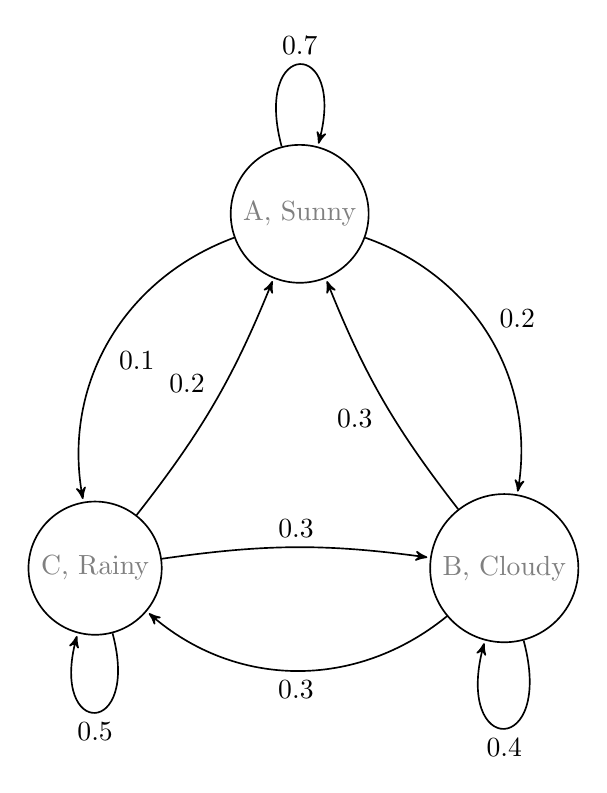
\begin{tikzpicture}[->, >=stealth', shorten >=1pt, auto, node distance=5cm, semithick]
        \tikzstyle{every state}=[fill=white,draw=black,text=gray]
    
        \node[state] (A) at (90:3cm) {A, Sunny};
        \node[state] (B) at (330:3cm) {B, Cloudy};
        \node[state] (C) at (210:3cm) {C, Rainy};
        
        \path (A) edge [loop above] node {0.7} (A)
                            edge [bend left=40] node {0.2} (B)
                            edge [bend right=40] node {0.1} (C)
                    (B) edge [bend left=8] node {0.3} (A)
                            edge [loop below] node {0.4} (B)
                            edge [bend left=40] node {0.3} (C)
                    (C) edge [bend right=8] node {0.2} (A)
                            edge [bend left=8] node {0.3} (B)
                            edge [loop below] node {0.5} (C);
    \end{tikzpicture}
    \end{center}

Following the example above, we can say, for instance, that the probability of moving from "Sunny" to "Sunny" is $0.7$, the probability of moving from "Sunny" to "Cloudy" is $0.2$, and so on..

\subsection{State at time $n$}
We have a beautiful MC that responds to Markov property, we have the transition matrix, we have the state transition graph, we have everything. Now we want to know, let's say, what's the state of the chain at time $n$?

Well, that's quite easy algebraically. We can use the transition matrix to calculate the state of the chain at any time $n$.
Let's say we have a toy MC with $$\mathbb{S} = \{0, 1, 2\}$$ and the transition matrix is: $$P = \begin{bmatrix} 0.7 & 0.2 & 0.1 \\ 0.3 & 0.4 & 0.3 \\ 0.2 & 0.3 & 0.5 \end{bmatrix}$$
We also know something we call "initial distribution" that is the probability distribution of the states at time $0$. Let's say that the initial distribution\footnote{The initial distribution is a vector of the same dimension as $|\mathbb{S}|$ that represents the probability for the chain to start at time $t = 0$ in a specific state.} is: $$\alpha_0 = \begin{bmatrix} 0.3 & 0.4 & 0.3 \end{bmatrix}$$

Now we questioning: "What's the state of the chain at time $n = 3$?".
We can calculate it using the transition matrix and the initial distribution. 

The state of the chain at time $n$ is given by:
$$\alpha_n = \alpha_0 \cdot P^n$$
Where: \begin{itemize}
    \item $\alpha_n$ is the probability distribution of the states at time $n$, it's a vector in which each entry represents the probability of being in a specific state at time $n$. For instance, if $\alpha_n[2] = 0.4$, it means that the probability of being in state $2$ at time $n$ is $0.4$. 
    \item $\alpha_0$ is the initial distribution as said before.
    \item $P$ is the transition matrix.
    \item $P^n$ is the transition matrix raised to the power of $n$. This represents the probability of moving from one state to another in $n$ steps.
\end{itemize}
This is called the "N-step transition probability of the chain".

\subsection{Stationary Distribution}
As for random variables, MC follow a sort of law of large numbers. If you keep flipping a coin for a long time, the proportion of heads and tails will eventually stabilize at 0.5 each. 

The same concept applies to MC. If you keep running a MC for a long time, the proportion of time spent in each state will eventually stabilize. This stable distribution is called the stationary distribution.

The stationary can be intended also as the long-term behavior of the chain. Or the limit of $t$ that goes to infinity. Mathematically:
$$\lim_{n \to \infty} \alpha_n = \pi$$
Where: \begin{itemize}
    \item $\pi$ is the stationary distribution.
    \item $\alpha_n$ is the probability distribution of the states at time $n$.
\end{itemize}

\paragraph{How do we compute this $\pi$?} Well, we can compute the stationary distribution by solving a system of linear equations. The stationary distribution $\pi$ is the solution to the equation:
$$\pi = \pi \cdot P$$
Where: \begin{itemize}
    \item $\pi$ is the stationary distribution.
    \item $P$ is the transition matrix.
\end{itemize}

And moreover, the sum of the entries of the stationary distribution must be equal to $1$ as it represents a probability distribution.\footnote{AKA the normalizaiton constraint.}
$$\sum_{i \in \mathbb{S}} \pi_i = 1$$

Now let's look it in a more practical way. We want to compute this $\pi$ and for computing it we have to solve a system of two equations: 
$$ \begin{cases} 
    \pi = \pi  \cdot P \\
    \sum_{i \in \mathbb{S}} \pi_i = 1
\end{cases}$$
\begin{itemize}
    \item The first equation is the "balance equation", it represents the fact that the stationary distribution is unchanged by the transition matrix. You can see it as a proof that the stationary distribution is the distribution that the system reaches after a long time. 
    \item The second equation is the normalization constraint, it ensures that the sum of the entries of the stationary distribution is equal to $1$ as we want a probability distribution\footnote{..And we know that the sum of the probabilities of all possible outcomes must be equal to 1.}. 
\end{itemize}
    

Coming back to out toy MC:
The stationary distribution $\pi$ is the solution to the equation:\footnote{Remember that $\pi \cdot P$ is a matrix multiplication.}
$$\begin{cases} \pi = \pi \cdot P \\
    \pi_0 + \pi_1 + \pi_2 = 1
\end{cases}$$

\subsection{Proportion of time spent in each state}
The stationary distribution $\pi$ tells us the proportion of time that the chain spends in each state in the long run.
So after computing this system you actually have a vecton $\pi$ composed by the proportion of time that the chain spends in each state.\\
Let's say that $\pi[4] = 0.324$. 

It means that the state associated to the $4^{th}$ entry of the vector $\pi$ is visited $32.4\%$ of the time in the long run and moreover we have a probability of being in state 4 of $32.4\%$, again, in the long run.


\section{Poisson Processes}

A \textbf{Poisson process} is a stochastic process used to model the occurrence of random events over time. It’s defined by a single rate parameter $\lambda$, which represents the average number of events per unit of time.

\subsection{When do we use Poisson vs Exponential?}
In a Poisson process:
\begin{itemize}
    \item \textbf{Poisson random variables:} These are used to count \textbf{how many events} happen in a fixed time interval. 
    For example, the number of events in a time interval of length $t$ is:
    \[
    N(t) \sim Pois(\lambda t),
    \]
    where $\lambda$ is the rate of events per unit time.
    So, how many events happened in $t$? That's a Poisson random variable with parameter $t$ times $\lambda$.

    \item \textbf{Exponential random variables:} These are used to model \textbf{when events happen}, specifically the time between consecutive events (called "inter-arrival times"). 
    The time between events follows an exponential distribution:
    \[
    T \sim Exp(\lambda).
    \]
    Where $T$ is the time between events, and $\lambda$ is the rate of events per unit time.
    So every event is separated by an amount of time that follows an exponential random variable with parameter $\lambda$, and never change, and has no memory!
\end{itemize}


In summary, Poisson counts \textbf{how many events}, while Exponential tells us \textbf{when events happen}.

\paragraph{Exponential RVs} EXP RVs has cool properties: \begin{itemize}
    \item \textbf{Memoryless Property}: The time until the next event is independent of how much time has already passed. $$P(T > s + t | T > s) = P(T > t)$$
    \item \textbf{Additivity Property}: The sum of independent exponential random variables is Gamma distributed. $$X_1 \sim Exp(\lambda_1), X_2 \sim Exp(\lambda_2) \implies X_1 + X_2 \sim Gamma(2, \lambda_1 + \lambda_2)$$ Where 2 is the number of summed exponential random variables and the second argument is the sum of their rate parameters.
    \item \textbf{Minimum Property}: The minimum of two exponential random variables is also exponential. $$X_1 \sim Exp(\lambda_1), X_2 \sim Exp(\lambda_2) \implies \min(X_1, X_2) \sim Exp(\lambda_1 + \lambda_2)$$ So to find which event happens first, you actually come up with an exponential random variable with the sum of the rate parameters.
\end{itemize}


\section{WIP CTM}

... \\
... \\



















\end{document}






\subsection{X Random Variable}
blabla
$$X \sim pippo(params)$$
blabla
\begin{itemize}
    \item Distribution function: 
    \item Expected value:
    \item Variance:
\end{itemize}

\newpage
\section{Appendix}
\noindent\begin{minipage}{\textwidth}
    \hrule
    \vspace{0.3cm}
    \paragraph{}
    \paragraph{}
    \vspace{0.3cm}
    \hrule
    \end{minipage}
    



\end{document}